% \textbf{\underline{OZ 5 - Magnetische inductie en de wet van Faraday - Oefening 3:}}
% \vspace{0.5cm}

% Een geïsoleerde draad wordt vervormd tot een acht zoals aangegeven in Figuur 5.3. De straal van de bovenste cirkel is 5,00 cm, de straal van de onderste is 9,00 cm. De draad heeft een uniforme weerstand per lengte-eenheid van 3,00 $ \Omega $/m. Een uniform magnetisch veld wordt aangelegd loodrecht op het vlak van de twee cirkels. De richting is aangegeven in de figuur. Dit magnetische veld groeit met 2,00 T/s. Bepaal de grootte en richting van de geïnduceerde stroom in de draad.

% \begin{figure}[H]
%     \centering
%     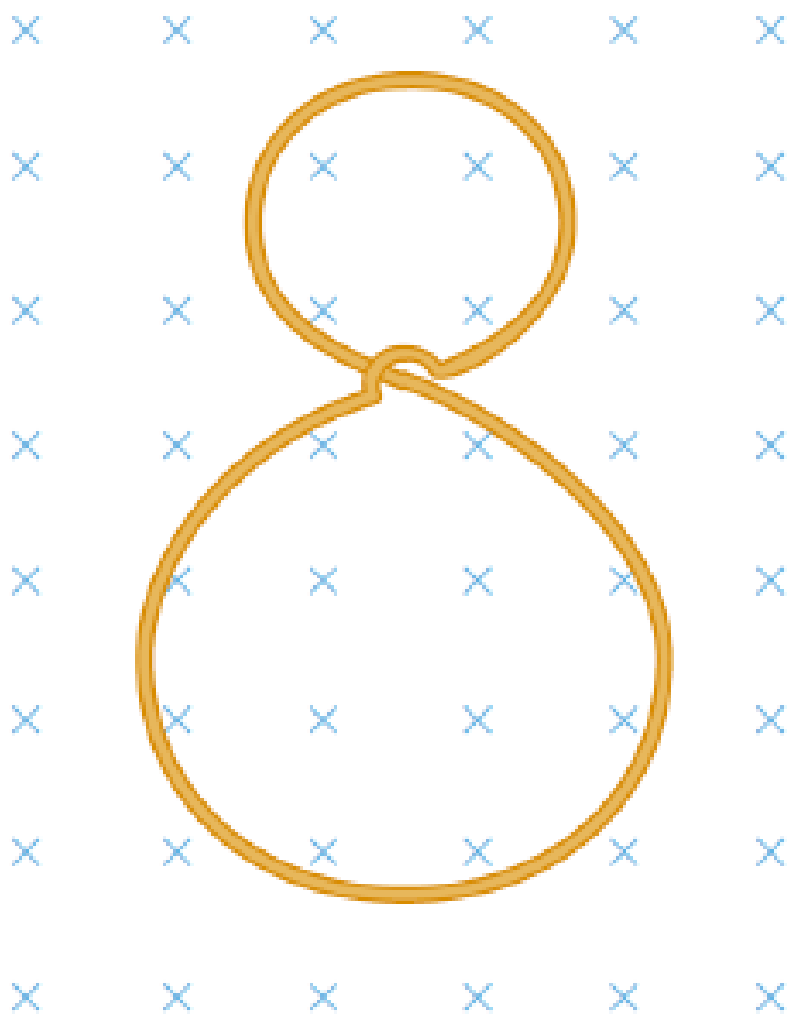
\includegraphics[width=4cm]{oz05/resources/oef-3-opgave.png}
    
%     \textbf{Figuur 5.3}
% \end{figure}

% \begin{description}[labelwidth=1.5cm, leftmargin=!]
%     \item[Geg. :]   $ r_1 = 5,00 $ cm; $ r_2 = 9,00 $ cm; $ \dfrac{dR}{dl} = 3,00 \ \Omega$/m; $ \dfrac{dB}{dt} = 2,00 $ T/s;
    
%     \item[Gevr. :]  $ \vec{I} $;
%     \item[Opl. :]   $ \dfrac{dB}{dt} = 2,00 $
    
%                     \hspace{-0.57cm} $ \Leftrightarrow
%                     dB = 2,00 dt $ 
    
%                     \hspace{-0.57cm} $ \Rightarrow
%                     \int_{0}^{B}{dB} = \int_{0}^{t}{2,00 dt} $ 
    
%                     \hspace{-0.57cm} $ \Leftrightarrow
%                     B = 2,00 t $ 
                    
%                     \vspace{0.5cm}
    
%                     $ \Phi_{B,1} = \int \vec{B} \cdot d\vec{A}_1 = B \cdot A_1 \cdot \cos{0^{\circ}} = 2,00 t \cdot \pi \cdot r_1^2  $
    
%                     \hspace{-0.57cm} $ \Rightarrow 
%                     \dfrac{d\Phi_{B,1}}{dt} = 2,00 \cdot \pi \cdot r_1^2 = 2,00 \cdot \pi \cdot (5,00 \cdot 10^{-2})^2 = \dfrac{\pi}{200} $ Wb/s
                    
%                     $ \varepsilon_1 = - \dfrac{d\Phi_{B,1}}{dt} = - \dfrac{\pi}{200} $ Wb/s
                    
%                     $ R_1 = \dfrac{dR}{dl} \cdot 2 \pi \cdot r_1 = 3,00 \cdot 2 \cdot \pi \cdot 5,00 \cdot 10^{-2} = \dfrac{3 \pi}{10} \ \Omega $ 
                    
%                     $ I_1 = \dfrac{\varepsilon_1}{R_1} = \dfrac{-\dfrac{\pi}{200}}{\dfrac{3 \pi}{10}} = -0,01667 $ A
                    
%                     \vspace{0.5cm}
                    
%                     $ \Phi_{B,2} = \int \vec{B} \cdot d\vec{A}_2 = B \cdot A_2 \cdot \cos{0^{\circ}} = 2,00 t \cdot \pi \cdot r_2^2  $
    
%                     \hspace{-0.57cm} $ \Rightarrow 
%                     \dfrac{d\Phi_{B,2}}{dt} = 2,00 \cdot \pi \cdot r_2^2 = 2,00 \cdot \pi \cdot (9,00 \cdot 10^{-2})^2 = \dfrac{81\pi}{5000} $ Wb/s
                    
%                     $ \varepsilon_2 = - \dfrac{d\Phi_{B,2}}{dt} = - \dfrac{81\pi}{5000} $ Wb/s
                    
%                     $ R_2 = \dfrac{dR}{dl} \cdot 2 \pi \cdot r_2 = 3,00 \cdot 2 \cdot \pi \cdot 9,00 \cdot 10^{-2} = \dfrac{27 \pi}{50} \ \Omega $ 
                    
%                     $ I_2 = \dfrac{\varepsilon_2}{R_2} = \dfrac{-\dfrac{81\pi}{5000}}{\dfrac{27 \pi}{50}} = -0,03 $ A
                    
%                     \vspace{0.5cm}
                    
%                     $ I = I_1 - I_2 = -0,01667 - \left( -0,03 \right) = 0,01333 $ A $ \approx 0,0133 $ A
% \end{description}

% \vspace{1cm}